\documentclass{beamer}
\usetheme{Frankfurt}
\usepackage{array,multirow,graphicx}
\usepackage{listings}

\title{Game Theory}
\subtitle{Lecture 15 \\ Computer Security DD2395}
\author[R. Guanciale]{
  Roberto Guanciale\\
  robertog@kth.se
}
\date{2015-12-15}
\begin{document}

\begin{frame}[plain]
  \titlepage
\end{frame}

\begin{frame}{Video Games}
  \begin{center}
    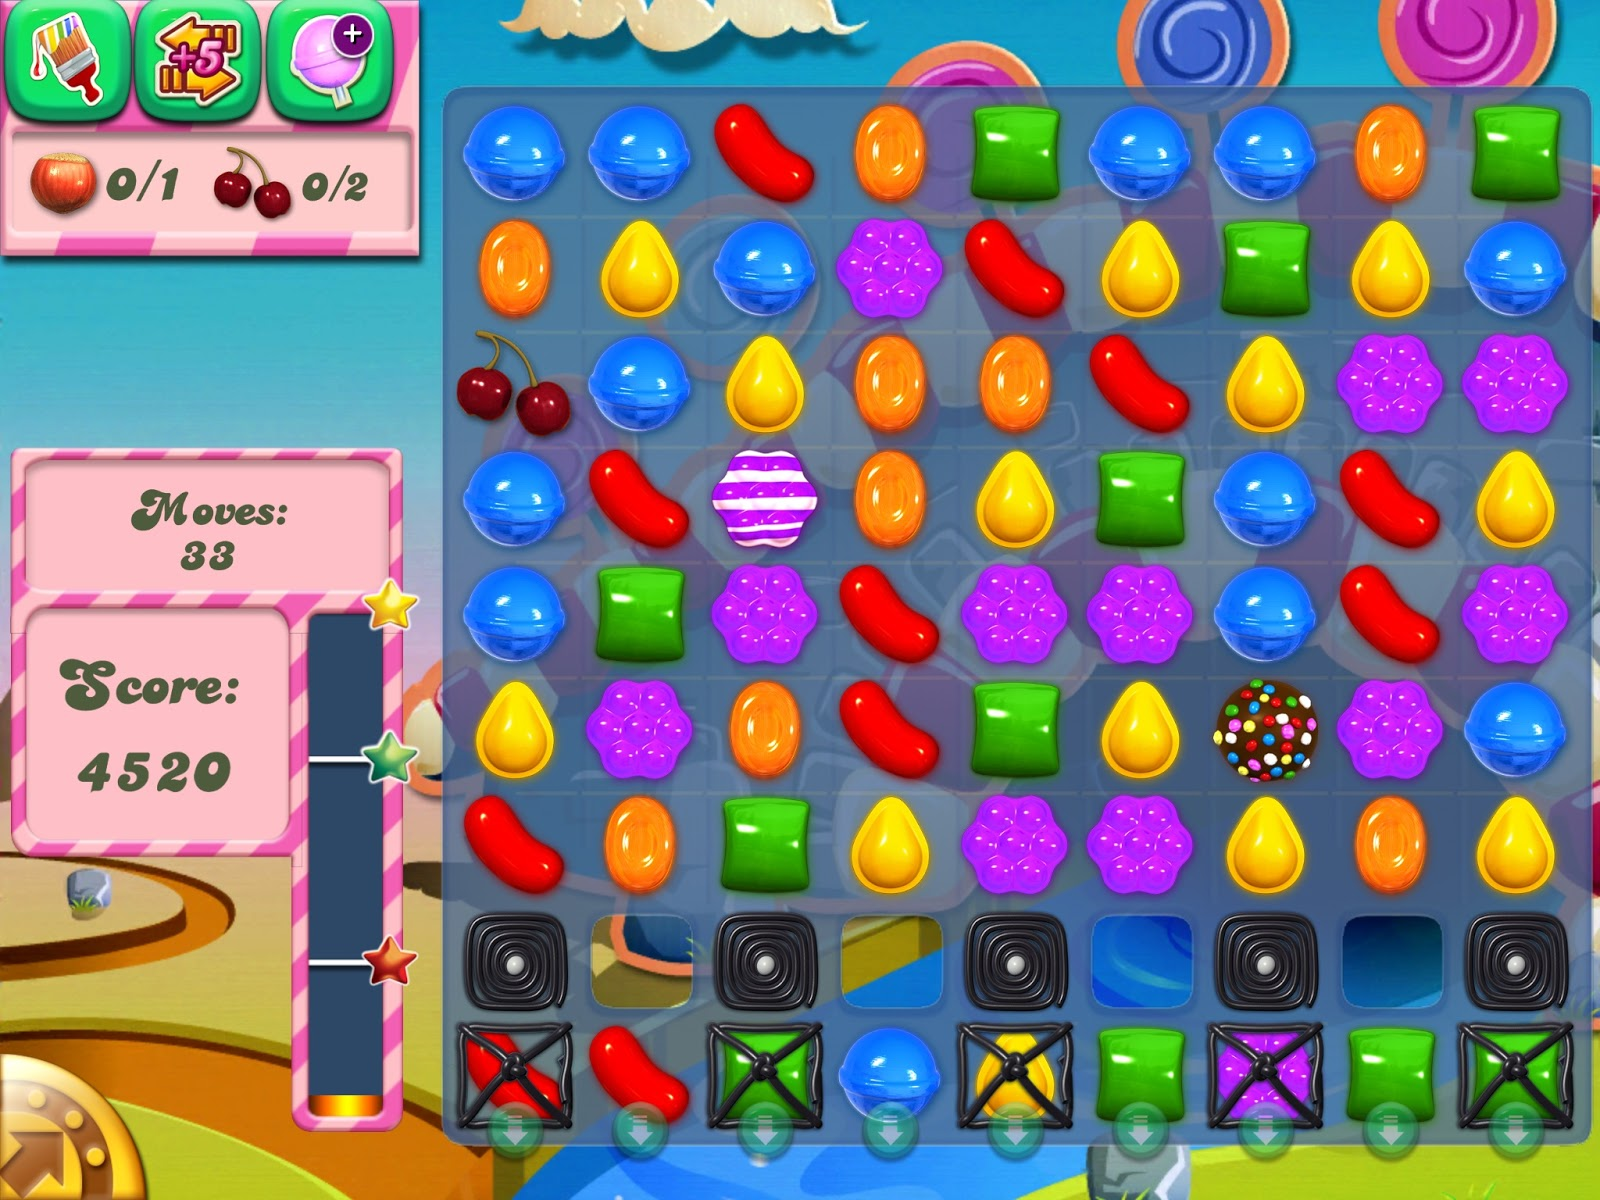
\includegraphics[width=0.4\linewidth]{candy}
    ~
    
\includegraphics[width=0.4\linewidth]{wow}
  \end{center}
  \begin{itemize}
    \item<2-> Game theory is not about this
    \item<3-> Game theory is ``the study of mathematical models of
      conflict and cooperation between intelligent rational
      decision-makers.''
    \item<4-> Why we can trust someone?
    \item<5-> How we can induce someone to be trustworthy?
  \end{itemize}
\end{frame}

\begin{frame}{The grading game}
  We play this game
  \begin{itemize}
    \item New rules for grading
    \item Without showing your neighbor what you are doing,
      write down on a form either the letter $\alpha$ or the letter
      $\beta$.
    \item I will randomly pair your
      form with one other form.
    \item Neither you nor your pair will ever know with whom you
      were paired.
    \item Here is how grades may be assigned for this course
      \begin{itemize}
      \item If you put $\alpha$ and your pair puts $\beta$ then you
        will get grade $A$, and your pair will fail the exam
      \item $\alpha$, $\alpha$ then both $E$
      \item $\beta$, $\beta$ then both $B$
      \item $\beta$, $\alpha$ then you fail, your pair $A$
      \end{itemize}
  \end{itemize}
\end{frame}

\begin{frame}{Terminology}
  \begin{itemize}
    \item The player choices $\alpha$ and $\beta$ are called strategies
    \item The final grades, e.g. (A, fail), are outcomes
  \end{itemize}
\begin{center}
  \begin{tabular}{|c|c|c|c|}
    \hline
    \multicolumn{4}{|c|}{Outcome Matrix}\\
    \hline
 &
&
\multicolumn{2}{|c|}{Strategy player pair}\\
    \hline
 & 
     & $\alpha$ & $\beta$  \\
    \hline
me & $\alpha$
     & E, E & A, fail \\
    \hline
 & $\beta$
     & fail, A & B,B \\
    \hline
  \end{tabular}
\end{center}
\end{frame}

\begin{frame}{Choosing a strategy}
  \begin{itemize}
  \item What strategy should a rational person choose?
  \item<2-> We need to know what that person cares about
  \item<3-> What ``payoff'' does each outcome yield for
    this person?
  \item<4-> Game theory can not tell us what payoff to assign to outcomes
  \item<4-> This depends on the preferences, moral sentiments
  \item<4-> Also depends on your opponents
  \item<5-> But game theory has a lot to say about how to play the game once payoff are known
  \end{itemize}
\end{frame}

\begin{frame}{Possible payoff: the selfish players}
\only<1>{
  \begin{itemize}
  \item every player is selfish and only cares
    about her own grade
  \end{itemize}
}
\begin{center}
  \begin{tabular}{|c|c|c|c|}
    \hline
    \multicolumn{4}{|c|}{Payoff Matrix 1}\\
    \hline
 &
&
\multicolumn{2}{|c|}{Strategy player pair}\\
    \hline
 & 
     & $\alpha$ & $\beta$  \\
    \hline
me & $\alpha$
     & 0,0 & 3, -5 \\
    \hline
 & $\beta$
     & -5, 3 & 2,2 \\
    \hline
  \end{tabular}
\end{center}
\only<2->{
  \begin{itemize}
  \item<2-> What should I choose in this case?
  \item<3-> If my pair chooses $\alpha$, then $\alpha$ gives me 0
    whereas $\beta$ gives me -5
  \item<4-> If my pair chooses $\beta$, then $\alpha$ gives me 3
    whereas $\beta$ gives me 2
  \item<5> So, in either case, choosing $\alpha$ is better
  \end{itemize}
}
\end{frame}

\begin{frame}{Definition}
  \begin{itemize}
  \item My strategy $\alpha$ ``strictly dominates'' my strategy
    $\beta$ if my payoff from $\alpha$ is strictly higher than that 
    from $\beta$ regardless of others' choice.
  \item<2-> $S_1$ ``strictly dominates'' $S_2$ for the player $i$ if
    for every other player $j$ and strategy $s^j$ (e.g.  $s^j \in \{\alpha, \beta\}$) holds
    $\textit{payoff}_i(s^1, \dots, s^{i-1}, S_1, s^{i+1}, \dots s^n) >
    \textit{payoff}_i(s^1, \dots, s^{i-1}, S_2, s^{i+1}, \dots s^n)$
  \item<3-> My strategy $\alpha$ ``weakly dominates'' my strategy
    $\beta$ if my payoff from $\alpha$ is as high than that 
    from $\beta$ regardless of others' choice and is strictly higher
    for at least one of such choice
  \item<4-> \textbf{You should never play a strictly dominated strategy}
  \end{itemize}
\end{frame}

\begin{frame}{Inefficiencies}
  \begin{itemize}
  \item You (if everyone is selfish) choose $\alpha$
  \item<2-> the reasoning is the same for your pair
  \item<3-> this leads to the outcome $(E,E)$, with payoff $(0,0)$
  \item<4-> while if both play $\beta$, the outcome $(B,B)$, with payoff $(2,2)$
  \item<5-> the outcome $(E,E)$ is called ``Pareto inefficient''
  \item<5-> \textbf{Rational play by rational players can lead to bad outcomes}
  \end{itemize}
\end{frame}

\begin{frame}{Applications}
  \begin{itemize}
  \item Prisoners' dilemma
  \item Price wars
  \item Remedies include: contracts enforced by the courts or by the
    organized crime
  \end{itemize}
\end{frame}

\begin{frame}{Possible payoff: the altruist players}
  \begin{itemize}
  \item each person cares also about the grade of the person with whom
    she is paired
  \item she like the grade A, but she feels guilty that this is at the
    expense of her pair failing
  \end{itemize}

\begin{center}
  \begin{tabular}{|c|c|c|c|}
    \hline
    \multicolumn{4}{|c|}{Payoff Selfish}\\
    \hline
 &
&
\multicolumn{2}{|c|}{Strategy player pair}\\
    \hline
 & 
     & $\alpha$ & $\beta$  \\
    \hline
me & $\alpha$
     & 0,0 & 3, -5 \\
    \hline
 & $\beta$
     & -5, 3 & 2,2 \\
    \hline
  \end{tabular}

  \begin{tabular}{|c|c|c|c|}
    \hline
    \multicolumn{4}{|c|}{Payoff Altruist}\\
    \hline
 &
&
\multicolumn{2}{|c|}{Strategy player pair}\\
    \hline
 & 
     & $\alpha$ & $\beta$  \\
    \hline
me & $\alpha$
     & 0,0 & -3, -5 \\
    \hline
 & $\beta$
     & -5, -3 & 2,2 \\
    \hline
  \end{tabular}
\end{center}

\end{frame}






\begin{frame}{Possible payoff: the selfish players}
\begin{center}
  \begin{tabular}{|c|c|c|c|}
    \hline
    \multicolumn{4}{|c|}{Payoff Altruist}\\
    \hline
 &
&
\multicolumn{2}{|c|}{Strategy player pair}\\
    \hline
 & 
     & $\alpha$ & $\beta$  \\
    \hline
me & $\alpha$
     & 0,0 & -3, -5 \\
    \hline
 & $\beta$
     & -5, -3 & 2,2 \\
    \hline
  \end{tabular}
\end{center}
  \begin{itemize}
  \item What should I choose in this case?
  \item<2-> If my pair chooses $\alpha$, then $\alpha$ gives me 0
    whereas $\beta$ gives me -5
  \item<3-> If my pair chooses $\beta$, then $\alpha$ gives me -3
    whereas $\beta$ gives me 2
  \item<4-> So, no strategy is dominated
  \item<5> To chose a strategy you should figure 
    out what are your payoffs (what do you care about)
    and what are other players' payoffs
  \end{itemize}
\end{frame}



\begin{frame}{The selfish vs the altruist}
  \begin{itemize}
  \item What if I am selfish but I know my opponent
    is altruist?
  \end{itemize}

\begin{center}
  \begin{tabular}{|c|c|c|c|}
    \hline
    \multicolumn{4}{|c|}{Payoff}\\
    \hline
 &
&
\multicolumn{2}{|c|}{Strategy player pair}\\
    \hline
 & 
     & $\alpha$ & $\beta$  \\
    \hline
me & $\alpha$
     & 0,0 & 3, -5 \\
    \hline
 & $\beta$
     & -5, -3 & 2,2 \\
    \hline
  \end{tabular}
\end{center}
\only<2>{
  \begin{itemize}
  \item My strategy $\alpha$ strictly dominates $\beta$
  \end{itemize}
}

\end{frame}


\begin{frame}{The altruist vs the selfish}
  \begin{itemize}
  \item What if I am altruist but I know my opponent
    is selfish?
  \end{itemize}

\begin{center}
  \begin{tabular}{|c|c|c|c|}
    \hline
    \multicolumn{4}{|c|}{Payoff}\\
    \hline
 &
&
\multicolumn{2}{|c|}{Strategy player pair}\\
    \hline
 & 
     & $\alpha$ & $\beta$  \\
    \hline
me & $\alpha$
     & 0,0 & -3, -5 \\
    \hline
 & $\beta$
     & -5, 3 & 2,2 \\
    \hline
  \end{tabular}
\end{center}
\only<2->{
  \begin{itemize}
  \item<2-> Neither of my strategies dominates the other
  \item<3-> My pair's strategy $\alpha$ strictly dominates her
    strategy $\beta$
  \item<4-> I should play $\alpha$ (to get $0 > -5$)
  \item<5-> If you do not have a dominated strategy,
    put yourself in your opponents' shoes to
    predict what they will do.
  \end{itemize}
}

\end{frame}

\begin{frame}{Open scenario}
  \begin{itemize}
  \item What if I do not know the payoffs of the person I am playing
    against?
  \item<2-> If I'm a selfish this is easy, $\alpha$ is always a
    dominating strategy
  \item<3-> If I am an altruist, it depends
    on what proportion (probability) of selfish and altruist
    I think there are in the population
    (``Bayesian games'')
  \item<4-> racist, classist, nationalist, sexist players
  \end{itemize}
\end{frame}

\begin{frame}{Real world example}
  \begin{itemize}
  \item What do real people do in Prisoners' Dilemmas?
  \item ``Normal people'' (no game theorist) about 30\% chose $\beta$
  \end{itemize}
\end{frame}

\begin{frame}{Nash equilibrium}
  \begin{itemize}
  \item Let $S = S_1 \times S_2 \times \dots \times S_n$ be the
    combination of all strategies of every player
  \item<2-> Let $x \in S$ be a strategy profile (an instance of the game)
  \item<3-> Let $f(x) = (f_1(x), f_2(x), \dots, f_n(x))$ be the payoff
    function
  \item<4-> Let $x_i$ be the strategy profile of $i$ and $x_{\bar i}$ be a
    strategy profile of all other players
  \item<5-> A strategy profile $x \in S$ is a Nash equilibrium
    if no unilateral deviation by any single player is profitable for
    that player
\[
  \forall i,x'_i\in S_i :  f_i(x_{i}, x_{\bar i}) \geq f_i(x'_{i},x_{\bar i}).
\]

  \end{itemize}
\end{frame}

\begin{frame}[t]{Stag hunt}
  \begin{itemize}
    \item two players may choose to hunt a stag or a rabbit
    \item stag provides more meat (4 units)
    \item rabbit provides less meat (1 unit)
    \item<2-> \textbf{the stag must be cooperatively hunted}
    \item<4-> two Nash equilibrium: (rabbit, rabbit) (stag, stag)
  \end{itemize}
  \only<3-> {
\begin{center}
  \begin{tabular}{|c|c|c|}
    \hline
     & stag & rabbit  \\
    \hline
stag
     & 2,2 & 0, 1 \\
    \hline
rabbit
     & 1,0 & 1,1 \\
    \hline
  \end{tabular}
\end{center}
}
\end{frame}

\begin{frame}[t]{Prisoner's dilemma}
  \begin{itemize}
    \item two prisoners held in separate cells, interrogated simultaneously
    \item ``cooperate'' (with the other prisoner) by not snitching
    \item ``defect'' by betraying the other
    \item<2-> \textbf{if only one defect, he obtains a huge benefit}
    \item<4->  The prisoner's dilemma has a single Nash equilibrium:
      both players defect
    \item<5->  climate-change / cold war
  \end{itemize}
  \only<3-> {
\begin{center}
  \begin{tabular}{|c|c|c|}
    \hline
              & cooperate & defect  \\
    \hline
cooperate     & -1,-1 & -5, 0 \\
    \hline
defect        & 0,-5 & -3,-3 \\
    \hline
  \end{tabular}
\end{center}
}
\end{frame}



\begin{frame}{Mechanism design}
  \begin{itemize}
    \item field in economics and game theory
    \item takes an engineering approach to designing economic
      mechanisms or incentives
    \item toward desired objectives
    \item where players act rationally
    \item can we force the players to do something?
    \item can we force the players to be truthful?
    \item how we can guarantee integrity of input provided by the parties?
  \end{itemize}
\end{frame}

\begin{frame}{Auction}
  \begin{itemize}
    \item a single, indivisible good is being sold
    \item $n$ buyers
    \item sealed-bid auction
    \item each buyer reports how much he is willing to pay
    \item<2-> the one with the highest price gets the good and pays
      the promised money
    \item<3-> $v_i$: real value of the buyer $i$
    \item<4-> $b_i$: bid of the buyer $i$
    \item<5-> payoff
\[
p_i(B) = \left \{
  \begin{array}{l}
    v_i - b_i \mbox{ if } b_i > max(B \setminus b_i)\\
    0         \mbox{ otherwise }
  \end{array}
\right .
\]
  \end{itemize}
\end{frame}


\begin{frame}{Auction}
\[
p_i(B) = \left \{
  \begin{array}{l}
    v_i - b_i \mbox{ if } b_i > max(B \setminus b_i)\\
    0         \mbox{ otherwise }
  \end{array}
\right .
\]
  \begin{itemize}
    \item there is no reason to bid $b_i > v_i$
    \item<2-> $p_i(v_i, b_{-i}) = 0$, there is no incentive to be trustworthy
    \item<3-> if $max(B \setminus b_i) > v_i$ (someone bids more the the value assigned by $i$) then 
      $p_i(b_i, b_{-i}) = p_i(v_i, b_{-i}) = 0$
    \item<4-> if $b_i < max(B \setminus b_i) < v_i$ ($j$ bids more the
      the bid of $i$) then 
      $p_i(b_i, b_{-i}) =  p_i(v_i, b_{-i}) = 0 < p_i(max(B \setminus
      b_i), b_{-i})$
    \item<5-> if $b_i > max(B \setminus b_i)$  then 
      $p_i(b_i, b_{-i}) >  p_i(v_i, b_{-i})$
  \end{itemize}
\end{frame}

\begin{frame}{Vickrey Auction}
  \begin{itemize}
    \item a single, indivisible good is being sold
    \item $n$ buyers
    \item sealed-bid auction
    \item each buyer reports how much he is willing to pay
    \item<2-> the one with the highest price gets the good and pays
      the second highest price
    \item<3-> payoff
\[
p_i(B) = \left \{
  \begin{array}{l}
    v_i - max(B \setminus b_i) \mbox{ if } b_i > max(B \setminus b_i)\\
    0         \mbox{ otherwise }
  \end{array}
\right .
\]
  \end{itemize}
\end{frame}


\begin{frame}{Vickrey Auction}
\[
p_i(B) = \left \{
  \begin{array}{l}
    v_i - max(B \setminus b_i) \mbox{ if } b_i > max(B \setminus b_i)\\
    0         \mbox{ otherwise }
  \end{array}
\right .
\]
  \begin{itemize}
    \item there is no reason to bid $b_i > v_i$
    \item<2-> if $max(B \setminus b_i) > v_i$ (someone bids more the the value assigned by $i$) then 
      $p_i(b_i, b_{-i}) = p_i(v_i, b_{-i}) = 0$
    \item<3-> if $b_i > max(B \setminus b_i)$  then 
      $p_i(b_i, b_{-i}) =  p_i(v_i, b_{-i}) = v_i - max(B \setminus b_i)$
    \item<4-> if $b_i < max(B \setminus b_i) < v_i$  then 
      $p_i(b_i, b_{-i}) =  0 < p_i(v_i, b_{-i}) = v_i - max(B
      \setminus b_i)$
    \item<5> \textbf{$b_i = v_i$ is a Nash equilibrium}
  \end{itemize}
\end{frame}


\begin{frame}{General mechanism design}
  \begin{itemize}
    \item There are $n$ players, having \emph{types} $\mathbf{t} = t_1, \dots, t_n$
    \item The type is a private information of the players
    \item Players report the types to the auctioneer
      $\mathbf{v} = v_1, \dots, v_n$
    \item A mechanism $\mathcal{M}(\mathbf{a},\mathbf{p})$ consists of two functions
      \begin{itemize}
      \item $\mathbf{a} = a_1(v_1), \dots , a_n(v_n)$ is the
        allocation vector (a probability vector in randomized games)
      \item $\mathbf{p} = p_1(v_1), \dots , p_n(v_n)$ is the payment
        vector
      \end{itemize}
    \item Player utility (payoff) $u_i(v_i \mid t_i) = a_i(\mathbf{v}) \circ
      t_i - p_i(\mathbf{v})$
    \item A mechanism is called truthful if $v_i = t_i$ is a dominant strategy
      equilibrium
  \end{itemize}
\end{frame}


\end{document}

%%% Local Variables: 
%%% mode: latex
%%% TeX-master: t
%%% End: 
